% !TEX encoding = UTF-8 Unicode
% !TEX program = xelatex

\documentclass{article}
	\usepackage[margin = 1.25in]{geometry}
	\usepackage{tikz}
	\usepackage{listings}
	\usepackage{fontspec}
\begin{document}



	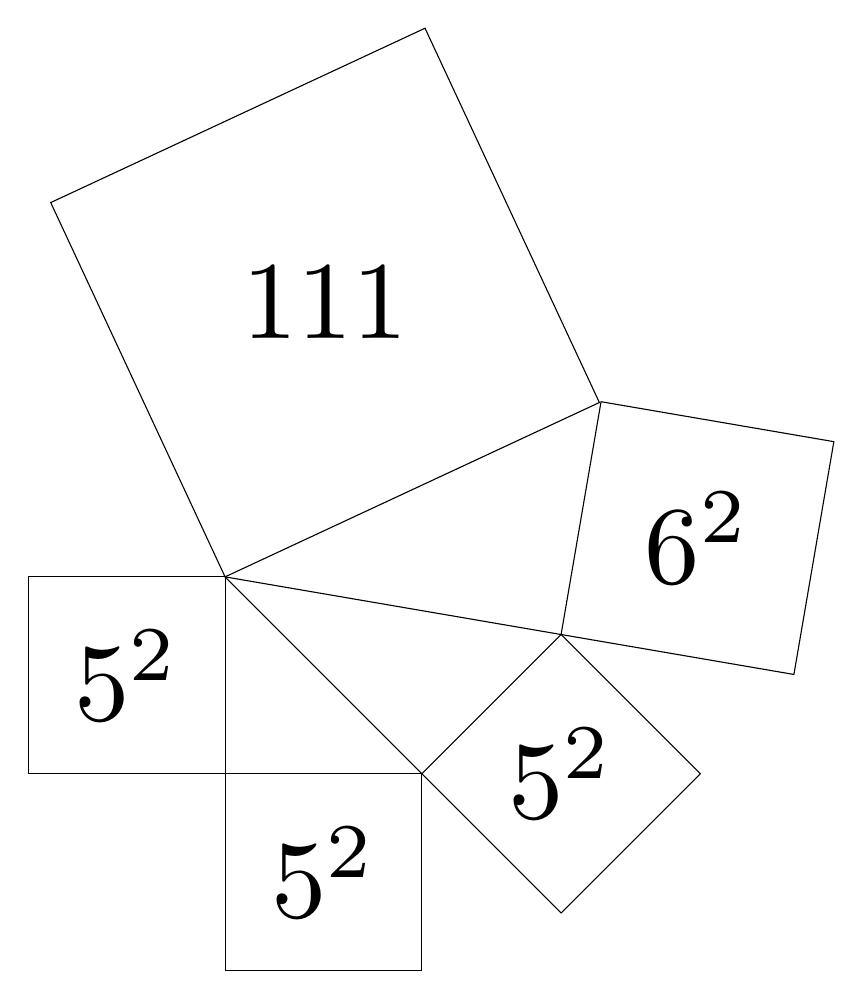
\begin{tikzpicture}[scale = 1/2,every node/.style = {scale = 4}]
		\draw (0, 0) rectangle node {$5^2$} (-5, -5) ;
		\draw (0, -5) rectangle node {$5^2$} (5, -10) ;
		\draw (0, 0) coordinate (orig) ;
		\draw [rotate = -45]
			(0, 0) -- ++({sqrt(50)}, 0) rectangle node{$5^2$} +(5, 5) ;
		\pgfmathsetmacro\gamma{atan2(5, sqrt(50))}
		\draw [rotate = -45 + \gamma]
			(0, 0) -- ++({sqrt(75)}, 0) rectangle node{$6^2$} +(6, 6) ;
		\pgfmathsetmacro\delta{atan2(6, sqrt(75))}
		\draw [rotate = -45 + \gamma + \delta]
			(0, 0) rectangle node {$111$} ({sqrt(110)}, {sqrt(110)}) ;
	\end{tikzpicture}



\fontspec{SourceCodePro-Regular}
\lstset{
	language=[latex]tex,tabsize=4,
	moredelim=*[s][\itshape]{$}{$},
	moredelim=*[s][\color{red!40!.}]{(}{)},
	moredelim=*[s][\color{green!30!.}]{[}{]},
	backgroundcolor=\color{blue!5},
	commentstyle=\color{.!80}\itshape,
	texcsstyle=*\color{blue!40!.},
	moretexcs={
		draw,pgfmathsetmacro
	},
	deletetexcs={},
}
%%%%%%%%%%%%%%%%%%%%%%%%%%%%%%%%%%%%%%%%%%%%%%%%%%%%%%%%%%%%%%%%%%%%%%%%%%%%%%%%
\begin{lstlisting}%%%%%%%%%%%%%%%%%%%%%%%%%%%%%%%%%%%%%%%%%%%%%%%%%%%%%%%%%%%%%%

% !TEX encoding = UTF-8 Unicode
% !TEX program = xelatex
\documentclass{article}
	\usepackage{tikz}
\begin{document}
	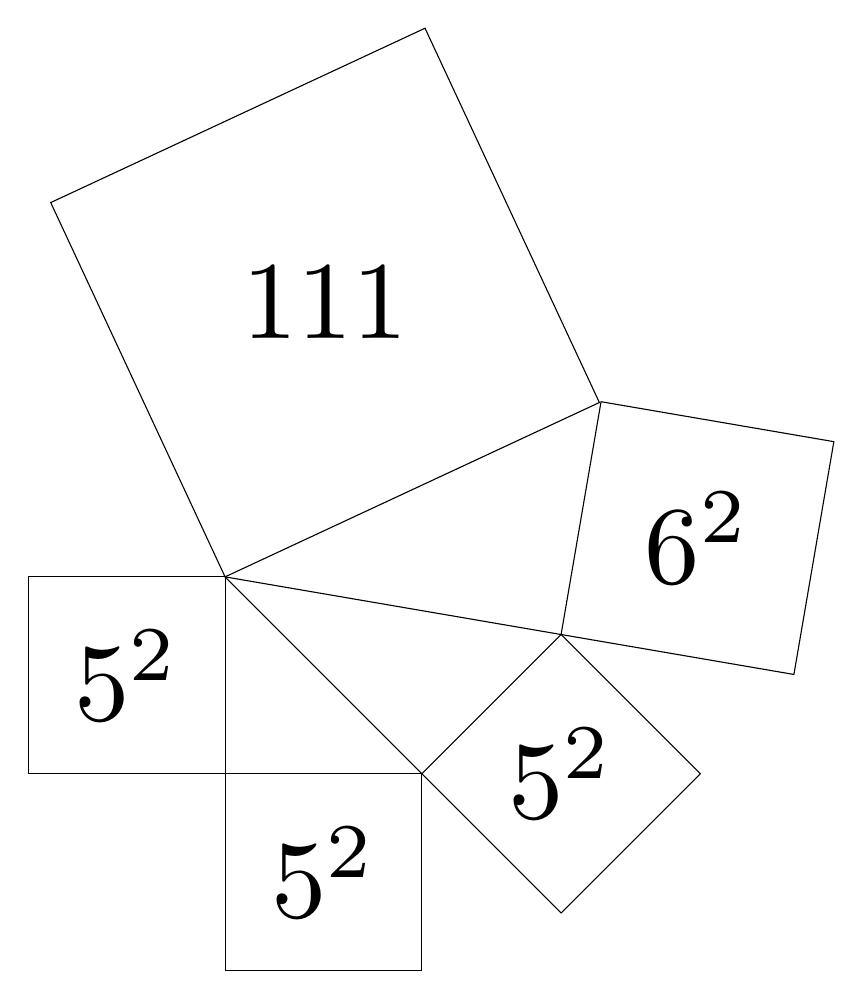
\begin{tikzpicture}[scale = 1/2,every node/.style = {scale = 4}]
		\draw (0, 0) rectangle node {$5^2$} (-5, -5) ;
		\draw (0, -5) rectangle node {$5^2$} (5, -10) ;
		\draw (0, 0) coordinate (orig) ;
		\draw [rotate = -45]
			(0, 0) -- ++({sqrt(50)}, 0) rectangle node{$5^2$} +(5, 5) ;
		\pgfmathsetmacro\gamma{atan2(5, sqrt(50))}
		\draw [rotate = -45 + \gamma]
			(0, 0) -- ++({sqrt(75)}, 0) rectangle node{$6^2$} +(6, 6) ;
		\pgfmathsetmacro\delta{atan2(6, sqrt(75))}
		\draw [rotate = -45 + \gamma + \delta]
			(0, 0) rectangle node {$111$} ({sqrt(110)}, {sqrt(110)}) ;
	\end{tikzpicture}
\end{document}

\end{lstlisting}%%%%%%%%%%%%%%%%%%%%%%%%%%%%%%%%%%%%%%%%%%%%%%%%%%%%%%%%%%%%%%%%
%%%%%%%%%%%%%%%%%%%%%%%%%%%%%%%%%%%%%%%%%%%%%%%%%%%%%%%%%%%%%%%%%%%%%%%%%%%%%%%%

\end{document}
